\documentclass[journal,12pt,onecolumn]{IEEEtran}
\usepackage{cite}
\usepackage{graphicx}
\usepackage{amsmath,amssymb,amsfonts,amsthm}
\usepackage{algorithmic}
\usepackage{graphicx}
\usepackage{textcomp}
\usepackage{xcolor}
\usepackage{txfonts}
\usepackage{listings}
\usepackage{enumitem}
\usepackage{mathtools}
\usepackage{gensymb}
\usepackage{comment}
\usepackage[breaklinks=true]{hyperref}
\usepackage{tkz-euclide} 
\usepackage{listings}
\usepackage{gvv}                                        
%\def\inputGnumericTable{}                                 
\usepackage[latin1]{inputenc} 
\usetikzlibrary{arrows.meta, positioning}
\usepackage{xparse}
\usepackage{color}                                            
\usepackage{array}                                            
\usepackage{longtable}                                       
\usepackage{calc}                                             
\usepackage{multirow}
\usepackage{multicol}
\usepackage{hhline}                                           
\usepackage{ifthen}                                           
\usepackage{lscape}
\usepackage{tabularx}
\usepackage{array}
\usepackage{float}
\newtheorem{theorem}{Theorem}[section]
\newtheorem{problem}{Problem}
\newtheorem{proposition}{Proposition}[section]
\newtheorem{lemma}{Lemma}[section]
\newtheorem{corollary}[theorem]{Corollary}
\newtheorem{example}{Example}[section]
\newtheorem{definition}[problem]{Definition}
\newcommand{\BEQA}{\begin{eqnarray}}
\newcommand{\EEQA}{\end{eqnarray}}
\usepackage{float}
%\newcommand{\define}{\stackrel{\triangle}{=}}
\theoremstyle{remark}
\usepackage{circuitikz}
\usepackage{tikz}
\title{GG: GEOLOGY AND GEOPHYSICS}
\author{EE25BTECH11032- KARTIK LAHOTI}
\begin{document}

\maketitle 

\begin{center}
    \subsection*{PART A: COMMON TO BOTH GEOLOGY AND GEOPHYSICS CANDIDATES}
\end{center}
\subsubsection*{Q.1 - Q.25 carry one mark each.}

    \begin{enumerate}
        \item The number of hydrous minerals in the Moh's scale of hardness is \rule{3cm}{0.15mm} \hfill{\brak{\text{GATE GG 2013}}}

        \item It takes approximately \rule{3cm}{0.15mm} minutes for sunlight to reach the Earth. \hfill{\brak{\text{GATE GG 2013}}}

        \item In a remotely sensed data of a planet, the presence of hydrous species can be inferred using \rule{3cm}{0.15mm} region of the electromagnetic spectrum? \hfill{\brak{\text{GATE GG 2013}}}
        \begin{enumerate}
            \begin{multicols}{4}
                \item Radiowave
                \item Gamma
                \item Infrared
                \item Visible
            \end{multicols}                    
        \end{enumerate}

        \item Amongst the following, which one will have the highest P-wave velocity? \hfill{\brak{\text{GATE GG 2013}}}
        \begin{enumerate}
            \begin{multicols}{4}
                \item Granite
                \item Diamond
                \item Shale
                \item Talc
            \end{multicols}
        \end{enumerate}

        \item Assuming the Earth to be a perfect sphere, its equatorial velocity is approximately \rule{3cm}{0.15mm}$\,km/hr$ \hfill{\brak{\text{GATE GG 2013}}}

        \item Both strength and plasticity of a rock increase with the \hfill{\brak{\text{GATE GG 2013}}}
            \begin{enumerate}
                \item increase in temperature
                \item decrease in strain rate
                \item increase in confining pressure
                \item increase in pore fluid pressure
            \end{enumerate}
            
        \item Amongst the following options, the acceptable value of the Poisson's ratio of a rock is \hfill{\brak{\text{GATE GG 2013}}}
            \begin{enumerate}
                \begin{multicols}{4}
                    \item $0.55$
                    \item $1.00$
                    \item $0.25$
                    \item $-1.00$
                \end{multicols}
            \end{enumerate}

        \item The acceleration due to gravity, $'g'$ is maximum at \hfill{\brak{\text{GATE GG 2013}}}
            \begin{enumerate}
                \begin{multicols}{4}
                    \item equator
                    \item poles
                    \item mid-latitudes
                    \item sub-tropical regions
                \end{multicols}
            \end{enumerate}

        \item The most abundant mineral in the Earth's crust is \hfill{\brak{\text{GATE GG 2013}}}
            \begin{enumerate}
                \begin{multicols}{4}
                    \item quartz
                    \item K-feldspar
                    \item biotite
                    \item garnet
                \end{multicols}
            \end{enumerate}

        \item Acoustic impedance is the \rule{3cm}{0.15mm} of density and velocity. \hfill{\brak{\text{GATE GG 2013}}}\hfill{\brak{\text{GATE GG 2013}}}
            \begin{enumerate}
                \begin{multicols}{4}
                    \item sum
                    \item difference
                    \item product
                    \item ratio
                \end{multicols}
            \end{enumerate}

        \item Choose the diamagnetic mineral from the following. \hfill{\brak{\text{GATE GG 2013}}}
            \begin{enumerate}
                \begin{multicols}{4}
                    \item Calcite
                    \item Enstatite
                    \item Pyrite
                    \item Ilmenite
                \end{multicols}
            \end{enumerate}

        \item Two bodies made up of same material with different dimensions have \hfill{\brak{\text{GATE GG 2013}}}
            \begin{enumerate}
                    \item same resistances and resistivities
                    \item same resistivities but different resistances
                    \item same resistances but different resistivities
                    \item different resistances and resistivities
            \end{enumerate}

        \item The type of wave that arrives first at a station from an earthquake hypocenter is \hfill{\brak{\text{GATE GG 2013}}}
            \begin{enumerate}
                \begin{multicols}{4}
                    \item P-wave
                    \item S-wave
                    \item Rayleigh wave
                    \item Love wave
                \end{multicols}
            \end{enumerate}

        \item Which one of the following is the correct statement? \hfill{\brak{\text{GATE GG 2013}}}
            \begin{enumerate}
                \item Accretionary wedge is part of the foreland basin
                \item Spreading ridge is a major zone of metamorphism
                \item Dehydration of subducting slab induces mantle melting
                \item Back arc basin represent a convergent regime
            \end{enumerate}
            
        \item Match the following items of \textbf{Group $I$} with those of \textbf{Group $II$}. \hfill{\brak{\text{GATE GG 2013}}}

        \begin{multicols}{2}
            \underline{\textbf{Group $I$}}
            \begin{enumerate}[start =16]
                \item Electrical Method
                \item Magnetic Method
                \item Gravity Method
                \item Seismic Method
            \end{enumerate}

            \columnbreak

            \underline{\textbf{Group $II$}}
            \begin{enumerate}
                \item Density
                \item Velocity
                \item Resistivity
                \item Susceptibility
                \item Dielectric Permittivity
            \end{enumerate}
        \end{multicols}

        \begin{enumerate}
            \item P-$3$, Q-$2$, R-$5$, S-$1$
            \item P-$3$, Q-$4$, R-$1$, S-$2$
            \item P-$3$, Q-$4$, R-$2$, S-$1$
            \item P-$5$, Q-$4$, R-$3$, S-$2$
        \end{enumerate}
        
        \item If a radioactive isotope has a decay constant of $1.55 \times 10^{-10}\text{year}^{-1}$, its half-life (in years) would be \hfill{\brak{\text{GATE GG 2013}}}
            \begin{enumerate}
                \begin{multicols}{4}
                    \item $4.57 \times 10^{9}$
                    \item $4.47 \times 10^{9}$
                    \item $4.57 \times 10^{10}$
                    \item $4.47 \times 10^{10}$
                \end{multicols}
            \end{enumerate}

        \item Which of the following physical properties of rocks has the widest range of variation? \hfill{\brak{\text{GATE GG 2013}}}
            \begin{enumerate}
                \begin{multicols}{2}
                    \item Magnetic permeability
                    \item Dielectric permittivity
                    \item Seismic velocity
                    \item Electrical resistivity
                \end{multicols}
            \end{enumerate}

        \item Which of the following is \underline{\textbf{NOT}} an inverse square law? \hfill{\brak{\text{GATE GG 2013}}}
            \begin{enumerate}
                    \item Newton's law of Gravitation
                    \item Coulomb's law of electrostatics
                    \item Coulomb's law of magnetostatics
                    \item Hooke's law
            \end{enumerate}
        
        \item A type of unconformity characterized by the occurrence of sedimentary rocks on igneous/metamorphic rocks is known as \hfill{\brak{\text{GATE GG 2013}}}
            \begin{enumerate}
                \begin{multicols}{2}
                    \item angular unconformity
                    \item nonconformity
                    \item paraconformity
                    \item disconformity
                \end{multicols}
            \end{enumerate}
        
        \item For seismic S-wave velocity, $V$, the rigidity modulus, $\mu$, is proportional to \hfill{\brak{\text{GATE GG 2013}}}
            \begin{enumerate}
                \begin{multicols}{4}
                    \item $\sqrt{V}$
                    \item $V$
                    \item $V^{2}$
                    \item $V^{3}$
                \end{multicols}
            \end{enumerate}

        \item An active trench is present in the vicinity of \hfill{\brak{\text{GATE GG 2013}}}
            \begin{enumerate}
                \begin{multicols}{2}
                    \item Andaman \& Nicobar Islands
                    \item Gulf of Cambay
                    \item Lakshadweep
                    \item Krishna-Godavari delta
                \end{multicols}
            \end{enumerate}

        \item In a homogeneous anisotropic medium, the physical property varies \hfill{\brak{\text{GATE GG 2013}}}
            \begin{enumerate}
                    \item with position but not with direction
                    \item with both position and direction
                    \item with direction but not with position
                    \item neither with position nor with direction
            \end{enumerate}
        \item Which one of the following stable isotopic ratios is used for estimation of palaeo-temperature of seawater? \hfill{\brak{\text{GATE GG 2013}}}
            \begin{enumerate}
                \begin{multicols}{2}
                    \item $^{13}\text{C/}^{12}\text{C}$
                    \item $^{18}\text{O/}^{16}\text{O}$
                    \item $^{87}\text{S/}^{86}\text{Sr}$
                    \item $^{15}\text{N/}^{14}\text{N}$
                \end{multicols}
            \end{enumerate}

        \item Match the following items of \textbf{Group $I$} with those of \textbf{Group $II$}. \hfill{\brak{\text{GATE GG 2013}}}

        \begin{multicols}{2}
            \underline{\textbf{Group $I$}}
            \begin{enumerate}[start =16]
                \item Coal
                \item Copper
                \item Oil
                \item Uranium
            \end{enumerate}

            \columnbreak

            \underline{\textbf{Group $II$}}
            \begin{enumerate}
                \item Gandhar
                \item Singareni
                \item Khetri
                \item Jadugoda
                \item Degana
            \end{enumerate}
        \end{multicols} 

        \begin{enumerate}
            \begin{multicols}{2}
                \item P-$4$, Q-$3$, R-$1$, S-$2$
                \item P-$2$, Q-$3$, R-$5$, S-$4$
                \item P-$1$, Q-$3$, R-$2$, S-$5$
                \item P-$2$, Q-$3$, R-$1$, S-$4$ 
            \end{multicols}            
        \end{enumerate}
        
        \item Which of the following logging techniques is best suited to estimate the shaliness of hydrocarbon reservoirs? \hfill{\brak{\text{GATE GG 2013}}}
            \begin{enumerate}
                \begin{multicols}{2}
                    \item Resistivity
                    \item Sonic
                    \item Induction
                    \item Gamma ray
                \end{multicols}
            \end{enumerate}

        \newpage

    \begin{center}
        \subsection*{PART B \brak{\text{SECTION 1}}: FOR GEOLOGY CANDIDATES ONLY}
    \end{center}
    
    \subsection*{Q.26 - Q.55 carry two mark each.}

        \item Which of the following statements is correct? \hfill{\brak{\text{GATE GG 2013}}}
            \begin{enumerate}
                \item Eolian sands do not exhibit cross bedding.
                \item Deep marine sands are well sorted.
                \item Glacier deposit may contain faceted pebble.
                \item Wave ripples do not form on shallow marine sands.
            \end{enumerate}

        \item The test of organic-walled foraminifera is termed as \hfill{\brak{\text{GATE GG 2013}}}
            \begin{enumerate}
                \begin{multicols}{2}
                    \item Microgranular
                    \item Hyaline
                    \item Porcellaneous
                    \item Tectinous
                \end{multicols}
            \end{enumerate}

        \item The void ratio (in percentage) of sandstone is $25$. Its porosity in percentage is \rule{3cm}{0.15mm}. \hfill{\brak{\text{GATE GG 2013}}}

        \item On a $1:10,000$ scale map, the length of a fault trace on a hrizontal plane is represented as $5\,cm$. The same on $1:25,000$ scale vertical aerial photograph is \rule{3cm}{0.15mm} $\,cm$ \hfill{\brak{\text{GATE GG 2013}}}

        \item In high-grade metamorphism, biotite melting indicates \hfill{\brak{\text{GATE GG 2013}}}
            \begin{enumerate}
                \begin{multicols}{2}
                    \item rock cooling
                    \item rock hydration
                    \item rock uplifting
                    \item rock dehydration
                \end{multicols}
            \end{enumerate}

        \item Match the defination type in \textbf{Group $I$} with the bivalves in \textbf{Group $II$}.\hfill{\brak{\text{GATE GG 2013}}}

        \begin{multicols}{2}
            \underline{\textbf{Group $I$}}
            \begin{enumerate}[start =16]
                \item Desmodont
                \item Dysodont
                \item Isodont
                \item Heterdont
            \end{enumerate}

            \columnbreak

            \underline{\textbf{Group $II$}}
            \begin{enumerate}
                \item \textit{Mytilus}
                \item \textit{Ceratoderma}
                \item \textit{Mya}
                \item \textit{Spondylus}
                \item \textit{Nucula}
                \item \textit{Arca}
            \end{enumerate}
        \end{multicols}

        \begin{enumerate}
            \begin{multicols}{2}
                \item P-$3$, Q-$1$, R-$4$, S-$2$
                \item P-$1$, Q-$2$, R-$6$, S-$5$
                \item P-$3$, Q-$1$, R-$5$, S-$2$
                \item P-$2$, Q-$1$, R-$4$, S-$6$
            \end{multicols}
        \end{enumerate}

        \item Which one of the following is the correct statement regarding hydrocarbon generation? \hfill{\brak{\text{GATE GG 2013}}}
            \begin{enumerate}
                \item H/C content of organic matter increases as it matures.
                \item O/C content of organic matter increases as it matures.
                \item Lignite does not form any hydrocarbon during maturation.
                \item Oil source rock is most abundant in Mesozoic.
            \end{enumerate}

        \item In the stereographic projection, $1$, $2$ and $3$ represent poles of three planes. Choose the correct combination of statements from the following.  \hfill{\brak{\text{GATE GG 2013}}}

        \begin{figure}[h]
	    \centering 	
            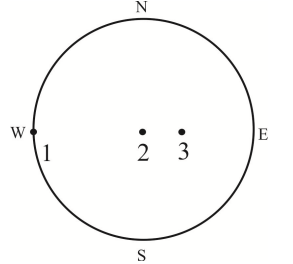
\includegraphics[width=0.5\columnwidth]{Figs/fig1.png}
            \caption{Question 33}
            \label{fig:placeholder_1}
        \end{figure}
        
            \begin{enumerate}
                \item The plane corresponding to $1$ is horizontal and the plane corresponding to $2$ is inclined.
                \item The plane corresponding to $1$ is striking N-S and the plane corresponding to 2 is horizontal.
                \item The plane corresponding to $2$ is vertical and the plane corresponding to $3$ is striking E-W.
                \item The plane corresponding to $2$ is striking E-W and the plane corresponding to $3$ is inclined.

            \end{enumerate}
\newpage
        \item Match the minerals in \textbf{Group $I$} with its corresponding industrial application in  \textbf{Group $II$}. \hfill{\brak{\text{GATE GG 2013}}}

        \begin{multicols}{2}
            \underline{\textbf{Group $I$}}
            \begin{enumerate}[start =16]
                \item Kaolinite
                \item Rutile
                \item Graphite
                \item Serpentine
            \end{enumerate}

            \columnbreak

            \underline{\textbf{Group $II$}}
            \begin{enumerate}
                \item Pigment
                \item Asbestos
                \item Cement
                \item Lubricant
                \item Abrasive
            \end{enumerate}
        \end{multicols}

        \begin{enumerate}
            \begin{multicols}{2}
                \item P-$1$, Q-$3$, R-$4$, S-$2$
                \item P-$3$, Q-$1$, R-$2$, S-$4$
                \item P-$3$, Q-$1$, R-$4$, S-$2$
                \item P-$1$, Q-$5$, R-$3$, S-$2$
            \end{multicols}
        \end{enumerate}

        \item  Match the Hermann-Maugin symbol in \textbf{Group $I$} with its corresponding general form in \textbf{Group $II$}. \hfill{\brak{\text{GATE GG 2013}}}
         
        \begin{multicols}{2}
            \underline{\textbf{Group $I$}}
            \begin{enumerate}[start =16]
                \item $6\text{/m}$
                \item $3\text{m}$
                \item $\overline{6}m^{2}$
                \item $\overline{6}$
            \end{enumerate}

            \columnbreak

            \underline{\textbf{Group $II$}}
            \begin{enumerate}
                \item Trigonal Dipyramid
                \item Ditrigonal Dipyramid
                \item Dihexagonal Pyramid
                \item Ditrigonal Pyramid
                \item Hexagonal Dipyramid
            \end{enumerate}
        \end{multicols}

        \begin{enumerate}
            \begin{multicols}{2}
                \item P-$5$, Q-$4$, R-$2$, S-$1$
                \item P-$5$, Q-$4$, R-$1$, S-$2$
                \item P-$5$, Q-$4$, R-$1$, S-$3$
                \item P-$3$, Q-$4$, R-$2$, S-$1$
            \end{multicols}
        \end{enumerate}

        \item Which of the following is a type of dam?\hfill{\brak{\text{GATE GG 2013}}}
            \begin{enumerate}
                \begin{multicols}{4}
                    \item Anchor
                    \item Shotcrete
                    \item Geogrid
                    \item Buttress
                \end{multicols}
            \end{enumerate}

        \item Match the following items in \textbf{Group $I$} with those in \textbf{Group $II$}. \hfill{\brak{\text{GATE GG 2013}}}

        \begin{multicols}{2}
            \underline{\textbf{Group $I$}}
            \begin{enumerate}[start =16]
                \item Kersantite
                \item Fenite
                \item Mugearite
                \item Phonolite
            \end{enumerate}

            \columnbreak

            \underline{\textbf{Group $II$}}
            \begin{enumerate}
                \item Hornblende-diopside-plagioclase lamprophyre
                \item Basaltic trachyandesite
                \item Volcanic nepheline syenite
                \item Biotite-plagioclase lamprophyre
                \item Metasomatic rock associated with carbonatites
            \end{enumerate}
        \end{multicols}

        \begin{enumerate}
            \begin{multicols}{2}
                \item P-$1$, Q-$2$, R-$4$, S-$3$
                \item P-$4$, Q-$5$, R-$2$, S-$3$
                \item P-$3$, Q-$1$, R-$2$, S-$4$
                \item P-$4$, Q-$5$, R-$3$, S-$2$
            \end{multicols}
        \end{enumerate}

         \item A chondrite-normalized REE pattern of quartzo-feldspathic gneiss shows a sharp positive
         $Eu$ anomaly. This indicates presence of  \hfill{\brak{\text{GATE GG 2013}}}
            \begin{enumerate}
                \item plagioclase in the sample.
                \item quartz in the sample.
                \item clinopyroxene in the sample.
                \item sillimanite in the sample.
            \end{enumerate}
            
        \item Choose the correct expression from the following that explains the changing vertical position of a point on the land surface at any time (Surface Uplift - SU, Bedrock Uplift - BU, Deposition - D, Compaction - C, Erosion - E). \hfill{\brak{\text{GATE GG 2013}}}
            \begin{enumerate}
                    \item $SU=BU-D-C-E$
                    \item $SU=BU-D+C-E$
                    \item $SU=BU+D-C+E$
                    \item $SU=BU+D-C-E$
            \end{enumerate}

        \item Match the following stratigraphic units listed in \textbf{Group $I$} with the Precambrian basins in \textbf{Group $II$}. \hfill{\brak{\text{GATE GG 2013}}}
            \begin{multicols}{2}
                \underline{\textbf{Group $I$}}
                \begin{enumerate}[start =16]
                    \item Badami Group
                    \item Kheinjua Formation
                    \item Sullavai Group
                    \item Papaghni Group
                \end{enumerate}
        
                \columnbreak
        
                \underline{\textbf{Group $II$}}
                \begin{enumerate}
                    \item Vindhyan
                    \item Chhatisgarh
                    \item Kaladgi
                    \item Cuddapah
                    \item Pranhita-Godavari
                \end{enumerate}
            \end{multicols}
            \begin{enumerate}
                \begin{multicols}{2}
                    \item P-$3$, Q-$1$, R-$5$, S-$4$
                    \item P-$1$, Q-$5$, R-$4$, S-$3$
                    \item P-$1$, Q-$2$, R-$3$, S-$5$
                    \item P-$3$, Q-$2$, R-$5$, S-$4$
                \end{multicols}
            \end{enumerate}

        \item Mantle xenoliths are observed in \hfill{\brak{\text{GATE GG 2013}}}
            \begin{enumerate}                
                    \item Kimberlite
                    \item Granite
                    \item Pegmatite
                    \item Granulite
            \end{enumerate}

        \item Dimension of hydraulic conductivity is \hfill{\brak{\text{GATE GG 2013}}}
            \begin{enumerate}
                \begin{multicols}{4}
                    \item $LT^{-2}$
                    \item $L^{3}T^{-1}$
                    \item $ML^{-3}$
                    \item $LT^{-1}$
                \end{multicols}
            \end{enumerate}

        \item Match the items in \textbf{Group $I$} with those in \textbf{Group $II$}. \hfill{\brak{\text{GATE GG 2013}}}
        \newpage
            \begin{multicols}{2}
                \underline{\textbf{Group $I$}}
                \begin{enumerate}[start=16]
                    \item Katrol Formation
                    \item Barail Formation
                    \item Ariyalur Formation
                    \item Sylhet Formation
                \end{enumerate}
        
                \columnbreak
        
                \underline{\textbf{Group $II$}}
                \begin{enumerate}
                    \item Oligocene
                    \item Cretaceous
                    \item Eocene
                    \item Jurassic
                    \item Paleocene
                    \item Miocene
                \end{enumerate}
            \end{multicols}
            \begin{enumerate}
                \begin{multicols}{2}
                        \item P-$2$, Q-$4$, R-$5$, S-$3$
                        \item P-$2$, Q-$5$, R-$3$, S-$1$
                        \item P-$4$, Q-$2$, R-$4$, S-$5$
                        \item P-$4$, Q-$1$, R-$2$, S-$3$
                \end{multicols}
            \end{enumerate}

        \item The outcrop pattern of folded sedimentary strata on the map given below represents \hfill{\brak{\text{GATE GG 2013}}}

        \begin{figure}[h]
	    \centering
            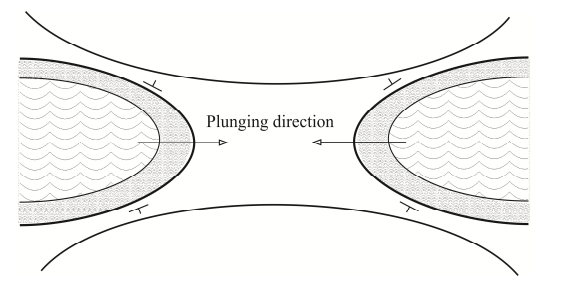
\includegraphics[width=0.5\columnwidth]{Figs/fig2.png}
            \caption{Question 44}
            \label{fig:placeholder_2}
        \end{figure}
        
            \begin{enumerate}
                \begin{multicols}{2}
                    \item culmination of antiform
                    \item culmination of synform
                    \item depression of antiform
                    \item depression of synform
                \end{multicols}
            \end{enumerate}

        \item Match the economic deposits in \textbf{Group $I$} with the host rocks in \textbf{Group $II$}. \hfill{\brak{\text{GATE GG 2013}}}
            \begin{multicols}{2}
                \underline{\textbf{Group $I$}}
                \begin{enumerate}[start=16]
                    \item Malanjkhand copper
                    \item Salem magnesite
                    \item Zawar Pb-Zn
                    \item Rampura-Agucha
                \end{enumerate}
        
                \columnbreak
        
                \underline{\textbf{Group $II$}}
                \begin{enumerate}
                    \item Granite
                    \item Dolomite
                    \item Graphitic Schist
                    \item Ultramafics
                    \item Basalt
                    \item Rhyollite
                \end{enumerate}
            \end{multicols}
            \begin{enumerate}
                \begin{multicols}{2}              
                        \item P-$1$, Q-$4$, R-$3$, S-$2$
                        \item P-$2$, Q-$3$, R-$5$, S-$2$
                        \item P-$1$, Q-$4$, R-$2$, S-$3$
                        \item P-$3$, Q-$2$, R-$6$, S-$5$
                \end{multicols}
            \end{enumerate}
\newpage
        \item The stereographic projection below shows the principal stress axes and fault planes. The projection represents a \hfill{\brak{\text{GATE GG 2013}}}

        \begin{figure}[h]
	    \centering
            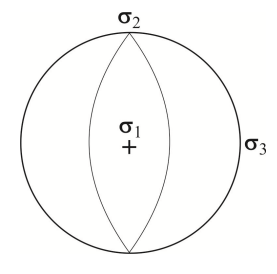
\includegraphics[width=0.5\columnwidth]{Figs/fig3.png}
            \caption{Question 46}
            \label{fig:placeholder_3}
        \end{figure}
        
            \begin{enumerate}
                \begin{multicols}{4}
                    \item normal fault
                    \item reverse fault
                    \item dextral fault
                    \item sinistral fault
                \end{multicols}
            \end{enumerate}
        \item Select the correct the statement from the following. \hfill{\brak{\text{GATE GG 2013}}}
            \begin{enumerate}
                \item Incised channels form an account of aeolin action.
                \item Mesa structures are observed only in steeply dipping beds.
                \item Crevasse splay is commonly associated with meandering river.
                \item Coral reefs are abundant in Gulf of Cambay.
            \end{enumerate}
            \newpage
\subsection*{Common Data Questions}
\subsubsection*{Common Data for Questions 48 and 49}

A, B, C, D, E, F and G are minerals in a sample of metamorphic rock. The micro-texture of the assemblage is given below. A, D and G are porphyroblasts, B and C are coronas, E and F are inclusions.

        \begin{figure}[h]
            \centering
            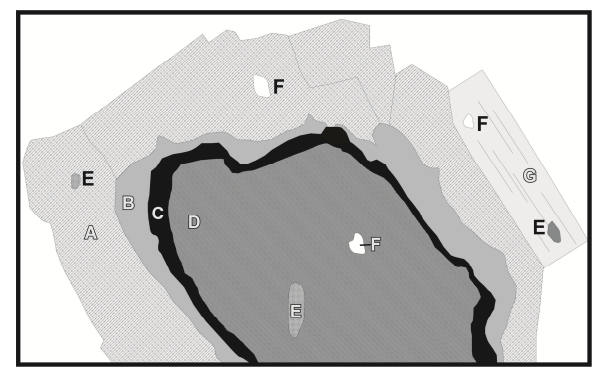
\includegraphics[width=1\columnwidth]{Figs/fig4.png}
            \caption{Common Data Questions 48 and 49}
            \label{fig:placeholder_4}
        \end{figure}

        \item Select the appropriate metamorphic reaction from the following options. \hfill{\brak{\text{GATE GG 2013}}}
            \begin{enumerate}
                \begin{multicols}{2}
                    \item $A + B = C + D$
                    \item $A + C = D + G$
                    \item $A + D = B + C$
                    \item $E + D = C + A$
                \end{multicols}
            \end{enumerate}

        \item Based on the micro-texture, select the oldest assemblage from the following. \hfill{\brak{\text{GATE GG 2013}}}
            \begin{enumerate}
                \begin{multicols}{4}
                    \item $A-D$
                    \item $E-F$
                    \item $B-C$
                    \item $A-G$
                \end{multicols}
            \end{enumerate}
    \newpage
\subsubsection*{Common Data for Questions 50 and 51}
The Mohr-Coulomb failure envolope $\brak{A-B}$ of a porous limestone is given below. 

        \begin{figure}[h]
            \centering
            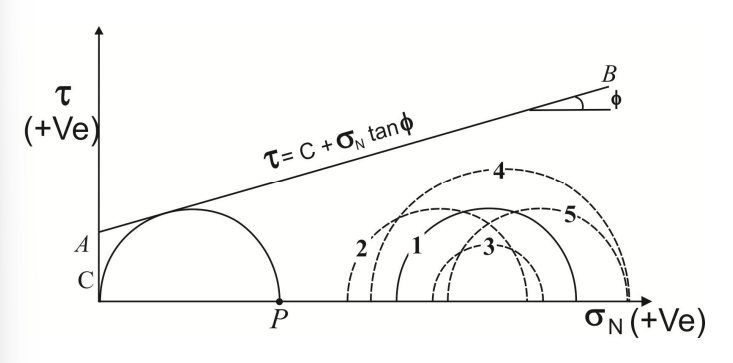
\includegraphics[width=1\columnwidth]{Figs/fig5.png}
            \caption{Common Data Questions 50 and 51}
            \label{fig:placeholder_5}
        \end{figure}

        \item The point P represents \hfill{\brak{\text{GATE GG 2013}}}
            \begin{enumerate}
                \item uniaxial tensile strength.
                \item uniaxial compressive strength.
                \item indirect tensile strength.
                \item shear strength.
            \end{enumerate}

        \item For a condition represented by the circle $1$, if pore water pressure increases, the circle will change to \hfill{\brak{\text{GATE GG 2013}}}
            \begin{enumerate}
                \begin{multicols}{4}
                    \item circle $2$.
                    \item circle $3$.
                    \item circle $4$.
                    \item circle $5$.
                \end{multicols}
            \end{enumerate}
\subsection*{Linked Answer Questions}
\subsubsection*{Statement for Linked Answer Questions 52 and 53}
Sedimentary structures are useful for determining the younging direction of a bed.

        \item Which one of the following sedimentary structure represents the bottom of a bed? \hfill{\brak{\text{GATE GG 2013}}}
            \begin{enumerate}
                \begin{multicols}{2}
                    \item Current crescent
                    \item Desiccation crack
                    \item Rain print
                    \item Load cast
                \end{multicols}
            \end{enumerate}

        \item Which sedimentary process is responsible for the generation of the structure identified above? \hfill{\brak{\text{GATE GG 2013}}}
            \begin{enumerate}
                \begin{multicols}{2}
                    \item Wave reworking
                    \item Liquefaction of sediments
                    \item Drying and desiccation
                    \item Erosion of cohesive substrate
                \end{multicols}
            \end{enumerate}
\subsubsection*{Statement for Linked Answer Questions 54 and 55}
    The table below represents recalculated cation compositions data of minerals.

    \begin{table}[H]
        \begin{center}
\begin{tabular}{ll}
    \textbf{Group I} & \textbf{Group II} \\
    P. Ferrite & 1. Hexagonal Close Packed (HCP) \\
    Q. Austenite & 2. Body Centered Cubic (BCC) \\
    R. Martensite & 3. Body Centered Tetragonal (BCT) \\
    & 4. Face Centered Cubic (FCC)
\end{tabular}
\end{center}
    \end{table}

        \item Select the correct garnet [$\brak{Ca,Fe,Mg,Mn}_3Al_2Si_3O_{12}$] and clinopyroxene [$Ca\brak{FeMg}Si_2O_6$] pair respectively. hfill{\brak{\text{GATE GG 2013}}}
            \begin{enumerate}
                \begin{multicols}{4}
                    \item $II$ and $III$
                    \item $II$ and $IV$
                    \item $I$ and $IV$
                    \item $I$ and $III$
                \end{multicols}
            \end{enumerate}
            
        \item Calculate the distribution coefficient [$K_D$] for the $Fe\text{-}Mg$ system. \hfill{\brak{\text{GATE GG 2013}}}
            \begin{enumerate}
                \begin{multicols}{4}
                    \item $0.504$
                    \item $0.620$
                    \item $1.420$
                    \item $1.535$
                \end{multicols}
            \end{enumerate}
    \newpage
\begin{center}
    \subsection*{PART B (SECTION 2): FOR GEOPHYSICS CANDIDATES ONLY }    
\end{center}
\end{enumerate}
\subsubsection*{Q.26 to Q.55 carry two marks each. }
        \begin{enumerate}[start = 26 ]
           
        \item A P-wave is reflected as both P- and S- waves from an interface at angles $r_p$ and $r_s$ respectively. The relationship between $r_p$ and $r_s$ is \hfill{\brak{\text{GATE GG 2013}}}
            \begin{enumerate}
                \begin{multicols}{4}
                    \item $r_p > r_s$
                    \item $r_p = r_s$
                    \item $r_p < r_s$
                    \item $r_p = 2r_s$
                \end{multicols}
            \end{enumerate}

        \item Which of the following ways of measuring the size of an earthquake does not require instrumental recording? \hfill{\brak{\text{GATE GG 2013}}}
            \begin{enumerate}
                \begin{multicols}{2}
                    \item Richter magnitude
                    \item Moment
                    \item $M_w$
                    \item Intensity
                \end{multicols}
            \end{enumerate}

        \item In what circumstances, the migrated reflection seismic section will be same as the unmigrated one? \hfill{\brak{\text{GATE GG 2013}}}
            \begin{enumerate}
                \begin{multicols}{2}
                    \item Inclined interfaces
                    \item Undulating interfaces
                    \item Horizontal interfaces
                    \item Vertical interfaces
                \end{multicols}
            \end{enumerate}

        \item Which of the following methods is best suited to estimate the resistivity variations in the upper mantle? \hfill{\brak{\text{GATE GG 2013}}}
            \begin{enumerate}
                    \item Deep electrical resistivity
                    \item Ground Penetrating Radar
                    \item Controlled Source Electromagnetics
                    \item Magnetotellurics
            \end{enumerate}

        \item Amongst the following $4$-electrode configurations of the electrical resistivity method, which is best suited for archeological investigations? \hfill{\brak{\text{GATE GG 2013}}}
            \begin{enumerate}
                    \item Schlumberger
                    \item Pole-Pole
                    \item Wenner
                    \item Dipole-Dipole
            \end{enumerate}

        \item A singular value of an $m \times n$ matrix, $A$, is defined as \hfill{\brak{\text{GATE GG 2013}}}
            \begin{enumerate}
                \begin{multicols}{2}
                    \item positive square root of eigenvalue of $AA^T$
                    \item modulus of eigenvalue of $A$
                    \item eigenvalue of $A^TA$
                    \item square of eigenvalue of $A$
                \end{multicols}
            \end{enumerate}

        \item In an ill-posed geophysical inverse problem, stated as non-singular matrix equation, the magnitude of determinant of the coefficient matrix is \hfill{\brak{\text{GATE GG 2013}}}
            \begin{enumerate}
                \begin{multicols}{4}
                    \item large
                    \item zero
                    \item near zero
                    \item very large
                \end{multicols}
            \end{enumerate}

        \item In a 4-layer subsurface model, which combination of A-, H-, K- and Q- type electrical resistivity sounding curves is \underline{\textbf{NOT}} possible? \hfill{\brak{\text{GATE GG 2013}}}
            \begin{enumerate}
                \begin{multicols}{4}
                    \item HA
                    \item AK
                    \item KQ
                    \item HQ
                \end{multicols}
            \end{enumerate}

        \item Which of the following characteristics of a Self Potential (SP) anomaly gives the approximate 
        position of centre of the buried ore body? \hfill{\brak{\text{GATE GG 2013}}}
            \begin{enumerate}
                \item Position of maximum of the anomaly
                \item Position of minimum of the anomaly
                \item Position of zero crossing
                \item Position midpoint between maximum and minimum of the anomaly
            \end{enumerate}

        \item Given a scalar function, $f(x,y) = xy$. The curl of gradient of $f(x,y)$ is \hfill{\brak{\text{GATE GG 2013}}}
            \begin{enumerate}
                \begin{multicols}{4}
                    \item $2x\,\hat{i}$
                    \item $-2y\,\hat{j}$
                    \item $0\,\hat{i}$
                    \item $x\,\hat{i} + y\,\hat{j}$
                \end{multicols}
            \end{enumerate}

        \item Which of the following is \underline{\textbf{NOT}} correct? \hfill{\brak{\text{GATE GG 2013}}}
            \begin{enumerate}
                \item In VLF-EM technique, the tilt-angle mode is best suited to locate conductive bodies
                \item Fraser filter is a difference filter
                \item Static shift affects MT impedance phase
                \item Tipper vector is derived from the three magnetic field components, $H_x, H_y$ and $H_z$.
            \end{enumerate}
        
        \item If L, B, F and T respectively stand for Latitude correction, Bouguer correction, Free-air correction and Terrain correction, then the order in which they will have to be applied for gravity data analysis is \hfill{\brak{\text{GATE GG 2013}}}
            \begin{enumerate}
                \begin{multicols}{4}
                    \item LFBT
                    \item LBTF
                    \item FLBT
                    \item TBLF
                \end{multicols}
            \end{enumerate}
        
        \item Geomagnetic secular variations originate from the \hfill{\brak{\text{GATE GG 2013}}}
            \begin{enumerate}
                \begin{multicols}{4}
                    \item inner core
                    \item outer core
                    \item crust
                    \item mantle
                \end{multicols}
            \end{enumerate}

        \item Removal of regional component from magnetic data is similar to \hfill{\brak{\text{GATE GG 2013}}}
            \begin{enumerate}
                    \item band-pass filtering
                    \item low-pass filtering
                    \item high-pass filtering
                    \item band-reject filtering
            \end{enumerate}
        
        \item Which of the following is useful to estimate the depth to the centre of a spherical body from a gravity anomaly curve? \hfill{\brak{\text{GATE GG 2013}}}
            \begin{enumerate}
                    \item Surface integration
                    \item Volume integration
                    \item Twice the absolute maximum
                    \item Half-width of the anomaly
            \end{enumerate}
        
        \item Application of reduction-to-pole technique to a magnetic anomaly results in \hfill{\brak{\text{GATE GG 2013}}}
            \begin{enumerate}
                \item flattening the anomaly curve.
                \item transforming the asymmetry in the anomaly to symmetry.
                \item halving the amplitude.
                \item doubling the amplitude.
            \end{enumerate}

        \item The Fourier transform of a comb function is \hfill{\brak{\text{GATE GG 2013}}}
            \begin{enumerate}
                \begin{multicols}{4}
                    \item delta function
                    \item comb function
                    \item sync function
                    \item rectangular function
                \end{multicols}
            \end{enumerate}
        
        \item In Cartesian coordinate system, if the geological strike of a two-dimensional body is oriented along the $x$-direction, then the electromagnetic field components associated with TM mode of magnetotelluric method are \hfill{\brak{\text{GATE GG 2013}}}
            \begin{enumerate}
                \begin{multicols}{4}
                    \item $H_x, E_y \text{ and }E_z$
                    \item $E_x, H_y \text{ and }E_z$
                    \item $H_x, H_y \text{ and }E_z$
                    \item $E_x, H_y \text{ and }H_z$
                \end{multicols}
            \end{enumerate}
        
        \item A seismic signal is recorded in the frequency band $100-250 Hz$. While digitizing the signal, the sampling interval one should choose to avoid aliasing is \rule{3cm}{0.15mm} $ms$. \hfill{\brak{\text{GATE GG 2013}}}

        \item Wadati diagram is a plot of the difference in P- and S- wave arrival times against the arrival time of P-wave. It helps in estimating the \hfill{\brak{\text{GATE GG 2013}}}
            \begin{enumerate}
                \begin{multicols}{2}
                    \item velocity of P-wave.
                    \item velocity of S-wave.
                    \item time of occurrence of earthquake.
                    \item hypocenter of earthquake.
                \end{multicols}
            \end{enumerate}
        
        \item Match the items of \textbf{Group $I$} with those of \textbf{Group $II$} \hfill{\brak{\text{GATE GG 2013}}}
            \begin{multicols}{2}
                \underline{\textbf{Group $I$}}
                \begin{enumerate}[start = 1]
                    \item Caliper log
                    \item NMR log
                    \item Neutron log
                    \item SP log
                \end{enumerate}
                
                \columnbreak
                
                \underline{\textbf{Group $II$}}
                \begin{enumerate}
                    \item Permeability
                    \item Resistivity
                    \item Diameter
                    \item Velocity
                    \item Porosity
                \end{enumerate}
            \end{multicols}
            \begin{enumerate}
                \begin{multicols}{2}
                    \item P - $3$, Q - $4$, R - $2$, S - $5$
                    \item P - $3$, Q - $1$, R - $5$, S - $2$
                    \item P - $4$, Q - $2$, R - $4$, S - $3$
                    \item P - $1$, Q - $3$, R - $2$, S - $4$        
                \end{multicols}
            \end{enumerate}
            
        \item The most common hydrocarbon indicator is \hfill{\brak{\text{GATE GG 2013}}}
        \begin{enumerate}
            \begin{multicols}{4}
                    \item flat spot
                    \item dim spot
                    \item bright spot
                    \item velocity sag
            \end{multicols}
        \end{enumerate}
        
            
\subsection*{Common Data Questions}
\subsubsection*{Common Data for Questions 48 and 49}

A recursive filter $y_n$ is given by $y_n = 2x_n - 1.5x_{n-1} + y_{n-2}$.

        \item The order of $y_n$ is \rule{3cm}{0.15mm}. \hfill{\brak{\text{GATE GG 2013}}}
        
        \item The transfer function of $y_n$ in $z$-domain is \hfill{\brak{\text{GATE GG 2013}}}
            \begin{enumerate}
                \begin{multicols}{2}
                    \item $\frac{1-1.5z}{2-z^2}$
                    \item $\frac{1-z^{2}}{2-1.5z}$
                    \item $\frac{2+z^{2}}{1+1.5z}$
                    \item $\frac{2-1.5z}{1-z^{2}}$
                \end{multicols}
            \end{enumerate}

\subsubsection*{Common Data for Questions 50 and 51:}
In a linear inverse problem, the coefficient matrix, $A = \myvec{ 2.00 & 2.01 \\ 2.01 & 2.00 }$.

        \item The eigenvalues of $A$ are \hfill{\brak{\text{GATE GG 2013}}}
            \begin{enumerate}
                \begin{multicols}{4}
                    \item $\brak{4.01\,, -0.01}$
                    \item $\brak{-4.01\,,-0.01}$
                    \item $\brak{4.01\,,0.01}$
                    \item $\brak{-4.01\,,1.01}$
                \end{multicols}
            \end{enumerate}
        
        \item If the elements of A are expressed up to first decimal place only, then the number of possible solution(s) of the resulting inverse problem is \hfill{\brak{\text{GATE GG 2013}}}
            \begin{enumerate}
                \begin{multicols}{4}
                    \item $1$
                    \item $2$
                    \item $3$
                    \item $\infty$
                \end{multicols}
            \end{enumerate}

\subsection*{Linked Answer Questions}
\subsubsection*{Statement for Linked Answer Questions 52 and 53}
In an electrical resistivity sounding survey a current of $20 mA$ is passed through the current electrodes separated by a distance of $50 m$ and a voltage of $3 V$ is measured across the potential electrodes, separated by $10 m$.

        \item The above electrode configuration is known as \hfill{\brak{\text{GATE GG 2013}}}
            \begin{enumerate}
                    \item Schlumberger
                    \item Wenner
                    \item Pole-Dipole
                    \item Pole-Pole
            \end{enumerate}
        
        \item The apparent resistivity $\brak{\text{in }\Omega-m}$ for the above electrode configuration is close to \hfill{\brak{\text{GATE GG 2013}}}
            \begin{enumerate}
                \begin{multicols}{4}
                    \item $100$
                    \item $200$
                    \item $300$
                    \item $400$
                \end{multicols}
            \end{enumerate}

\subsubsection*{Statement for Linked Answer Questions 54 and 55:}
An electromagnetic (EM) wave of frequency $25 Hz$ is impinging on a homogeneous half-space, having resistivity of $100 \Omega-m$.

        \item The skin-depth of the wave is about \hfill{\brak{\text{GATE GG 2013}}}
            \begin{enumerate}
                \begin{multicols}{4}
                    \item $1 km$
                    \item $1 m$
                    \item $500 km$
                    \item $500 m$
                \end{multicols}
            \end{enumerate}
        
        \item The velocity of the EM wave $\brak{\text{in} km/s}$ is close to \hfill{\brak{\text{GATE GG 2013}}}
            \begin{enumerate}
                \begin{multicols}{2}
                    \item $20\pi$
                    \item $30\pi$
                    \item $40\pi$
                    \item $50\pi$
                \end{multicols}
            \end{enumerate}
            
\subsection*{General Aptitude (GA) Questions }    

\subsubsection{Q.56 to Q.60 carry one marks each. }

        \item A number is as much greater than $75$ as it is smaller than $117$. The number is: \hfill{\brak{\text{GATE GG 2013}}}
            \begin{enumerate}
                \begin{multicols}{4}
                    \item $91$
                    \item $93$
                    \item $89$
                    \item $96$
                \end{multicols}
            \end{enumerate}
            

        \item \underline{The professor} \underline{ordered to} \underline{ the students to go} \underline{out of the class}. \\\hspace{2cm}$I$\hspace{3cm}$II$\hspace{2.5cm}$III$\hspace{2cm}$IV$\\
        Which of the above underlined parts of the sentence is grammatically incorrect?\hfill{\brak{\text{GATE GG 2013}}}
        
            \begin{enumerate}
                
                    \begin{multicols}{4}
                    \item $I$
                    \item $II$
                    \item $III$
                    \item $IV$
                \end{multicols}
            \end{enumerate}

        \item Which of the following options is the closest in meaning to the word given below:
        \hfill{\brak{\text{GATE GG 2013}}}
            \begin{enumerate}
                \begin{multicols}{2}
                    \item Modern
                    \item Historic
                    \item Primitive
                    \item Antique
                \end{multicols}
            \end{enumerate}

        \item Friendship, no matter how \rule{3cm}{0.15mm} it is, has its limitations.\hfill{\brak{\text{GATE GG 2013}}}
            \begin{enumerate}
                    \item cordial
                    \item intimate
                    \item secret
                    \item pleasant
            \end{enumerate}

        \item Select the pair that best expresses a relationship similar to that expressed in the pair: \textbf{Medicine: Health} \hfill{\brak{\text{GATE GG 2013}}}
            \begin{enumerate}
                \begin{multicols}{2}
                    \item Science: Experiment
                    \item Wealth: Peace
                    \item Education: Knowledge
                    \item Money: Happiness
                \end{multicols}
            \end{enumerate}
\subsection{Q.61 to Q.65 carry two marks each. }

        \item $X \text{ and } Y$ are two posivtive numbers such that $2X + Y \leq 6 \text{ and } X + 2Y \leq 8$. For which of the following values of $\brak{X,Y}$ the function $f\brak{X,Y} = 3X + 6Y$ will give maximum value? \hfill{\brak{\text{GATE GG 2013}}}
            \begin{enumerate}
                \item $\brak{4/3\,, 10/3}$
                \item $\brak{8/3\,, 20/3}$
                \item $\brak{8/3\,, 10/3}$
                \item $\brak{4/3\,, 20/3}$
            \end{enumerate}
        \newpage
        \item If $\mydet{4X - 7} = 5$ then the values of $2\mydet{X} - \mydet{-X}$ is: \hfill{\brak{\text{GATE GG 2013}}}
            \begin{enumerate}
                \begin{multicols}{4}
                    \item $2\,, 1/3$
                    \item $1/2\,, 3$
                    \item $3/2\,, 9$
                    \item $2/3\,, 9$
                \end{multicols}
            \end{enumerate}

         \item Following table provides figures (in rupees) on annual expenditure of a firm for two years - $2010 \text{ and }2011$.   \hfill{\brak{\text{GATE GG 2013}}}
            \begin{table}[H]
                \centering
                \begin{tabular}{|c|c|c|}
     \hline
     \textbf{Mineral} & \textbf{Modal abundance \brak{\%}} & \textbf{Partition coefficient}\\
     \hline
     Clinopyroxene & $45$ & $0.506$ \\
      \hline
      Orthopyroxene & $40$ & $0.42$ \\
      \hline
      Olivine & $10$ & $0.045$ \\
      \hline
      Plagioclase & $05$ & $0.019$ \\
      \hline
\end{tabular}
            \end{table}

            In 2011, which of the following two categories have registered increase by same percentage?
            \begin{enumerate}
                \item Raw material and Salary \& wages
                \item Salary \& wages and Advertising
                \item Power \& fuel and Advertising
                \item Raw material and Research \& Development
            \end{enumerate}

        \item A firm is selling its product at $Rs. 60$ per unit. The total cost of production is $Rs. 100$ and firm is earning total profit of $Rs. 500$. Later, the total cost increased by $30\%$. By what percentage the price should be increased to maintained the same profit level. \hfill{\brak{\text{GATE GG 2013}}}
            \begin{enumerate}
                \begin{multicols}{4}
                    \item $5$
                    \item $10$
                    \item $15$
                    \item $30$
                \end{multicols}
            \end{enumerate}
        
         \item Abhishek is elder to Savar. Savar is younger to Anshul. Which of the given conclusions is logically valid and is inferred from the above statements? \hfill{\brak{\text{GATE GG 2013}}}
            \begin{enumerate}
                \item Abhishek is elder to Anshul
                \item Anshul is elder to Abhishek
                \item Abhishek and Anshul are of same age
                \item No conclusion follows
            \end{enumerate}

\begin{center}
    \subsection*{END OF THE QUESTION PAPER}
\end{center}

    
    \end{enumerate}
\end{document}

